\documentclass[letterpaper]{article}
\usepackage[margin=1.25in]{geometry}
\usepackage{amsmath}
\usepackage{amssymb}
\usepackage{titling}
\usepackage{graphicx}
\usepackage{caption} 
\usepackage{float}
\usepackage{subfig}
\usepackage{enumitem}
\usepackage{parskip}
\usepackage{titlesec}
\usepackage{mathtools}
\usepackage{url}


\allowdisplaybreaks
\title{
	\textbf{Politech Mathematical Group} \\ 
	\vspace{2ex} 
	Political Fatness Report
	\vspace{2ex}
}
\author{
	Darren Kong \\ 110770716
	\and 
	Hugo Mainguy \\ 111747982
	\and 
	Jeffrey Zhong \\ 112299792
	\vspace{3ex}
}
\date{March 5, 2021}

\begin{document}


\begin{titlepage}
\maketitle
\thispagestyle{empty}
\end{titlepage}

\section{Abstract}
%TODO%
%needs to be written (let’s aim for maybe 150 words max? Is that how people do this here?)%

\section{Introduction}

The advent of technology, especially in more recent times, has made every aspect of life “more” something. For instance, we are more connected with the Internet and instant communication across the globe than we were with letters, or printed newspapers. It may seem that this intensification of long-distance communication should make us all closer to one another. Yet, it seems that technology has also made mankind more divided, with the decentralization of news outlets or American politics. With the advent of technology, the decennial process of redistricting states with more than one congressional district has become a partisan affair. Fewer districts are competitive now than even twenty years ago (Cook) such that there is less need to appeal to the other side. Artificial intelligence applied to redistricting has contributed to a polarization of American politics; however, if used with good intentions, it could become the very solution to a problem that it fueled in the first place.

It is easy to call out gerrymandering, yet, at the same time, difficult to give precise measures for it. In Vieth v. Jubelirer, ruled in 2004, the Supreme Court argued that a districting was not gerrymandered for there was no measure to quantify inequality or lack of fairness. As courts – especially the Supreme Court – often rule by precedent, this has been used as an excuse to bring down some cases that made it to the highest court of the land. This has emboldened strategists to make increasingly “unfair” maps. The surge in gerrymandered districting plans is the combination of three factors that all came together at the same time: large political successes for one party, the Republicans, just before drawing districts, the sudden improvement of technology, and the increasing polarization in voting patterns. 

%Needs some sources for the claims here%

This comes together in what could be considered a paradox: while there are ever more accurate methods to gerrymander at will, there is no mathematical standard accepted by the courts to identify the practice as of today. Furthermore, state constitutions tend to lag even further behind, because of the amount of the slow legislative process and support required to change them. As explained by Levitt, only twenty-three states require their congressional districts to be contiguous. While in practice, this is virtually always the case, it creates more potential for gerrymandering in over half of the states. (Contiguity refers to the fact that any point of the district must be accessible from any other point of the district without leaving it, except for example if part of it is an island and there is a method of transportation such as a bridge or a regular ferry between both sides.) Furthermore, only eighteen states have any mention of compactness for their congressional districts. Within those eighteen states, a minority have more requirements. For instance, Iowa requests that districts not be oddly shaped (the state is almost a rectangle that can be split equally in four rectangles), California asks for districts not to bypass nearby large population areas for more distant populated areas, Arizona requires at least some of the districts to be competitive if feasible, and Rhode Island to represent the state fairly (although it currently has two congressional districts and will most likely lose one after the 2020 Census reapportionment.) Overall, there is a lot of leeway in what can be done by the redistricting committee. 


\section{Methodology}
To counter this, we suggest setting a standard with a definition of compactness. Compactness is something easily perceivable by humans, yet, there is no measure that satisfies human perception all the time - and we sometimes disagree among ourselves, as shown by Kaufman et al. 
However, a generally sensible choice is using the Polsby-Popper measure, which is given by the formula:

\[
	PP(D) = \frac{4\pi A(D)}{P(D)^2}
\]

% Need sources for these claims

Where A(D) is the area of the object D and P(D) its perimeter. This gives us a ratio between 0 and 1. It is 0 precisely when the area is 0 (D is a line or a point) and 1 when D is a circle. In particular, this favors compact round objects, and defavors those with longer or jagged perimeters. Both of these are important, and the measure has been used in real life, for instance with Arizona’s redistricting in 2000. It is noteworthy that several states use different measures, particularly in the West, where more attention is paid to fairness.
% Citation needed%
Other measures are used in different states: for instance, in Colorado, the districts should minimize the total perimeter. States like California and Michigan instead focus on dispersion rather than contorted boundaries, as Monorief points out. 

It becomes evidently clear that the Polsby Popper measure only takes into consideration the geometric compactness or fatness of the redistricting shape. A more suitable measure for compactness would also take into consideration the population requirement of the districtings. All congressional districtings have to be equal in population at the time of the redistricting. For example, a congressional district may seem to be shaped oddly but that is only due to the legal requirement for equal population size.

Simultaneously, it became clearer that while a non compact district is almost always subject to gerrymandering, the converse is not always true. One example of this is when districts bypass population centers nearby to instead include populations that are further away.
Here we will propose an alternative to the Polsby Popper that will be referred to as the Population Fatness measure, or Fatness for brevity. 
To calculate this measure, we used the following formula:

\[
	\frac{POP(\text{D})}{POP(\text{BC(D)})}
\]

Where D represents the district D, BC(D) is the minimum bounding circle that contains D, and POP(D) is the population in D. This measure utilizes precincts as the base level of a population cluster. Since the bounding circle cuts through some precincts, in those cases, the ratio of the area of the precinct in the circle is used to estimate the population of the part of the precinct inside of the bounding circle, yielding good approximations. Since precincts form districts, we do not need to apply any ratio other than 1 for the districts. Furthermore, this measure only takes into account the population that is inside the state, as the population outside of the state but inside the bounding circle should not influence the districts. Once again, a perfect score of 1 comes when the district is a perfect circle, and a low score close to 0 comes when the bounding circle encompasses many populous precincts, large areas of land, or a combination of both.

%[We should probably include the code for the two measures here, if anyone feels like adding it. Actually, maybe after each measure, whatever is better.]%

Since these two measures are different, it is interesting to compare them to see when they are similar and when they differ, explain why that is the case, and conclude whether those districts are gerrymandered or not. Using the current congressional districts, here are the data points found (Pennsylvania and North Carolina maps are from 2016).

\section{Results}

\begin{figure}[H]
	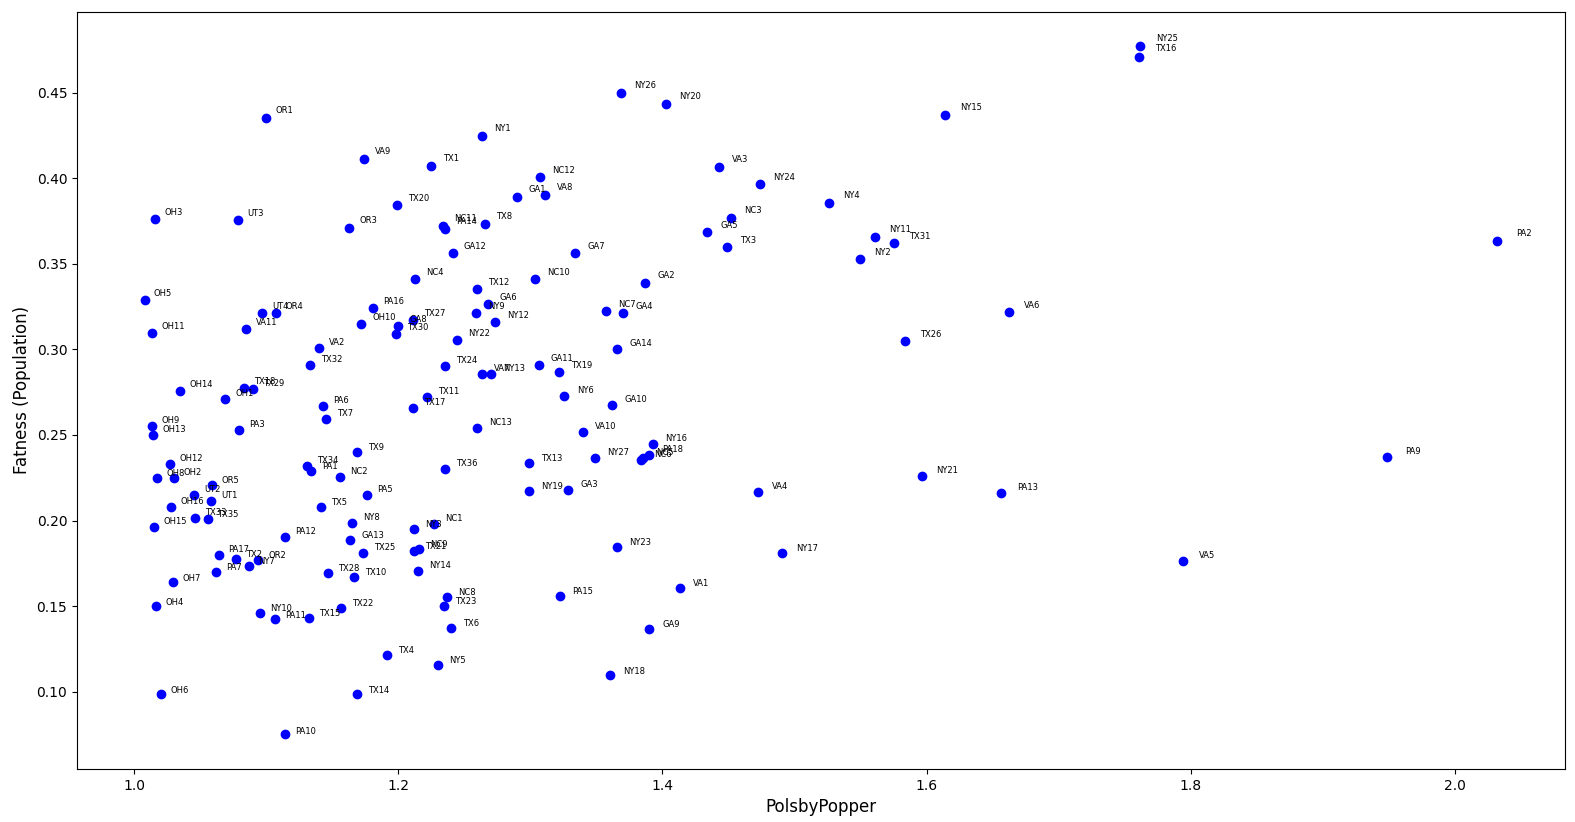
\includegraphics[width=\linewidth]{./figures/fatnessPopulationVpolsbyPopper.png}
	\caption{Plot of Population Fatness v. PolsbyPopper}
	\label{fig:datapoints}
\end{figure}

%We need a better name for this section
\section{Research}
From the results, we can see compare each district's Fatness score with its Polsby Popper score. To help easily identify specific districts, we will split the graph into four quadrants. The quadrants are to be referred from 1 to 4 starting from the top right in a counterclockwise fashion. We do this to identify extremeties in each of the district scores to see in what cases these two scores may differ wildly.

\begin{figure}[H]
	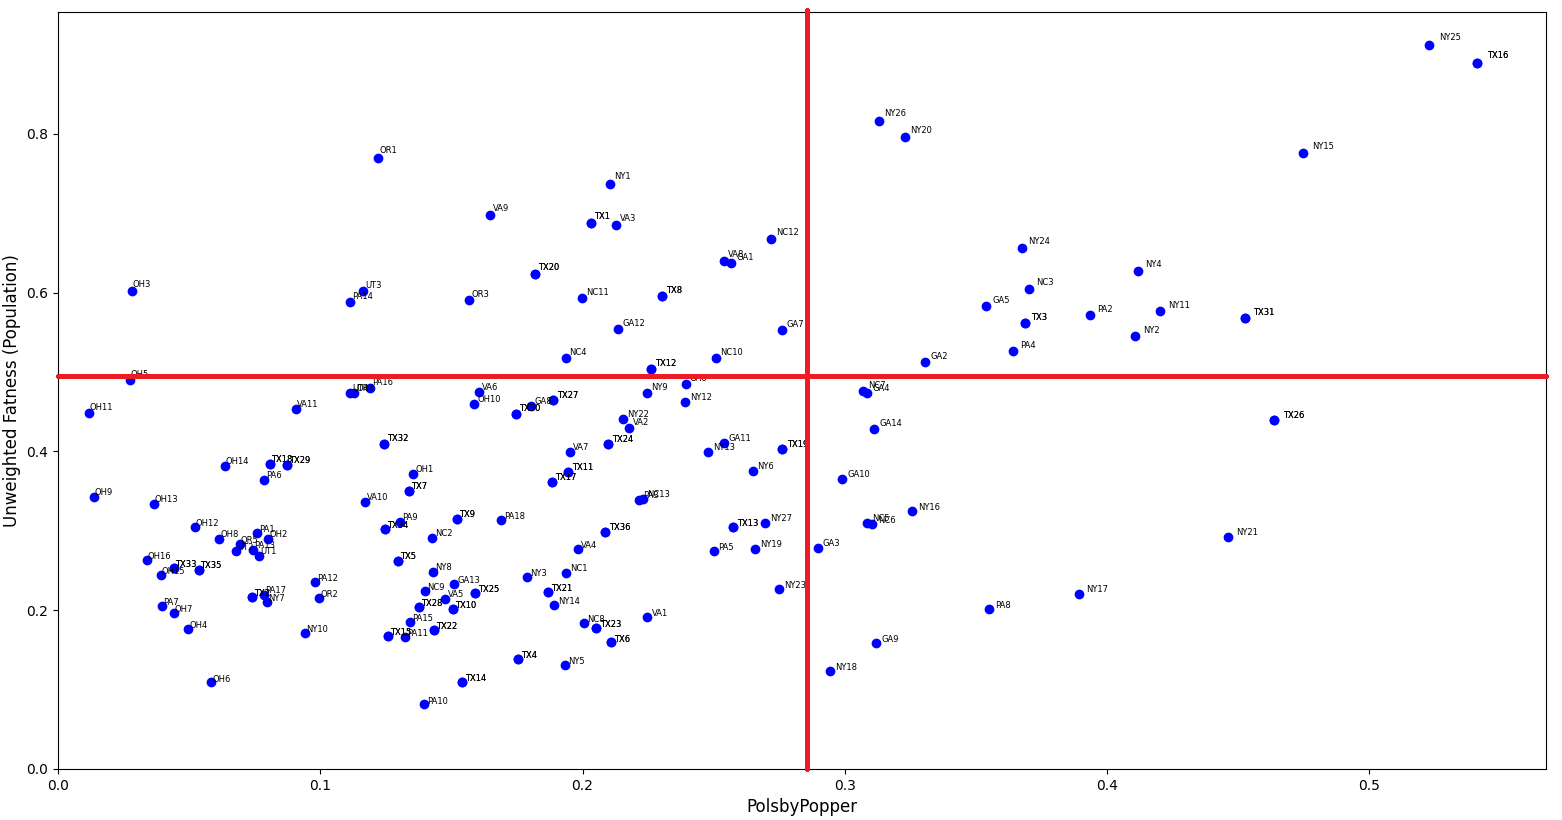
\includegraphics[width=\linewidth]{./figures/fatnessPopulationVpolsbyPopperEdited.png}
	\caption{Plot of Population Fatness v. PolsbyPopper Edited}
	\label{fig:datapointsEdited}
\end{figure}

We will begin our look on the first quadrant, specifically NY-25, NY-15, and TX-16. The district scores for both Fatness and Polsby Popper are both high for these districts. It is rather easy to tell why.

\begin{figure}[H]
	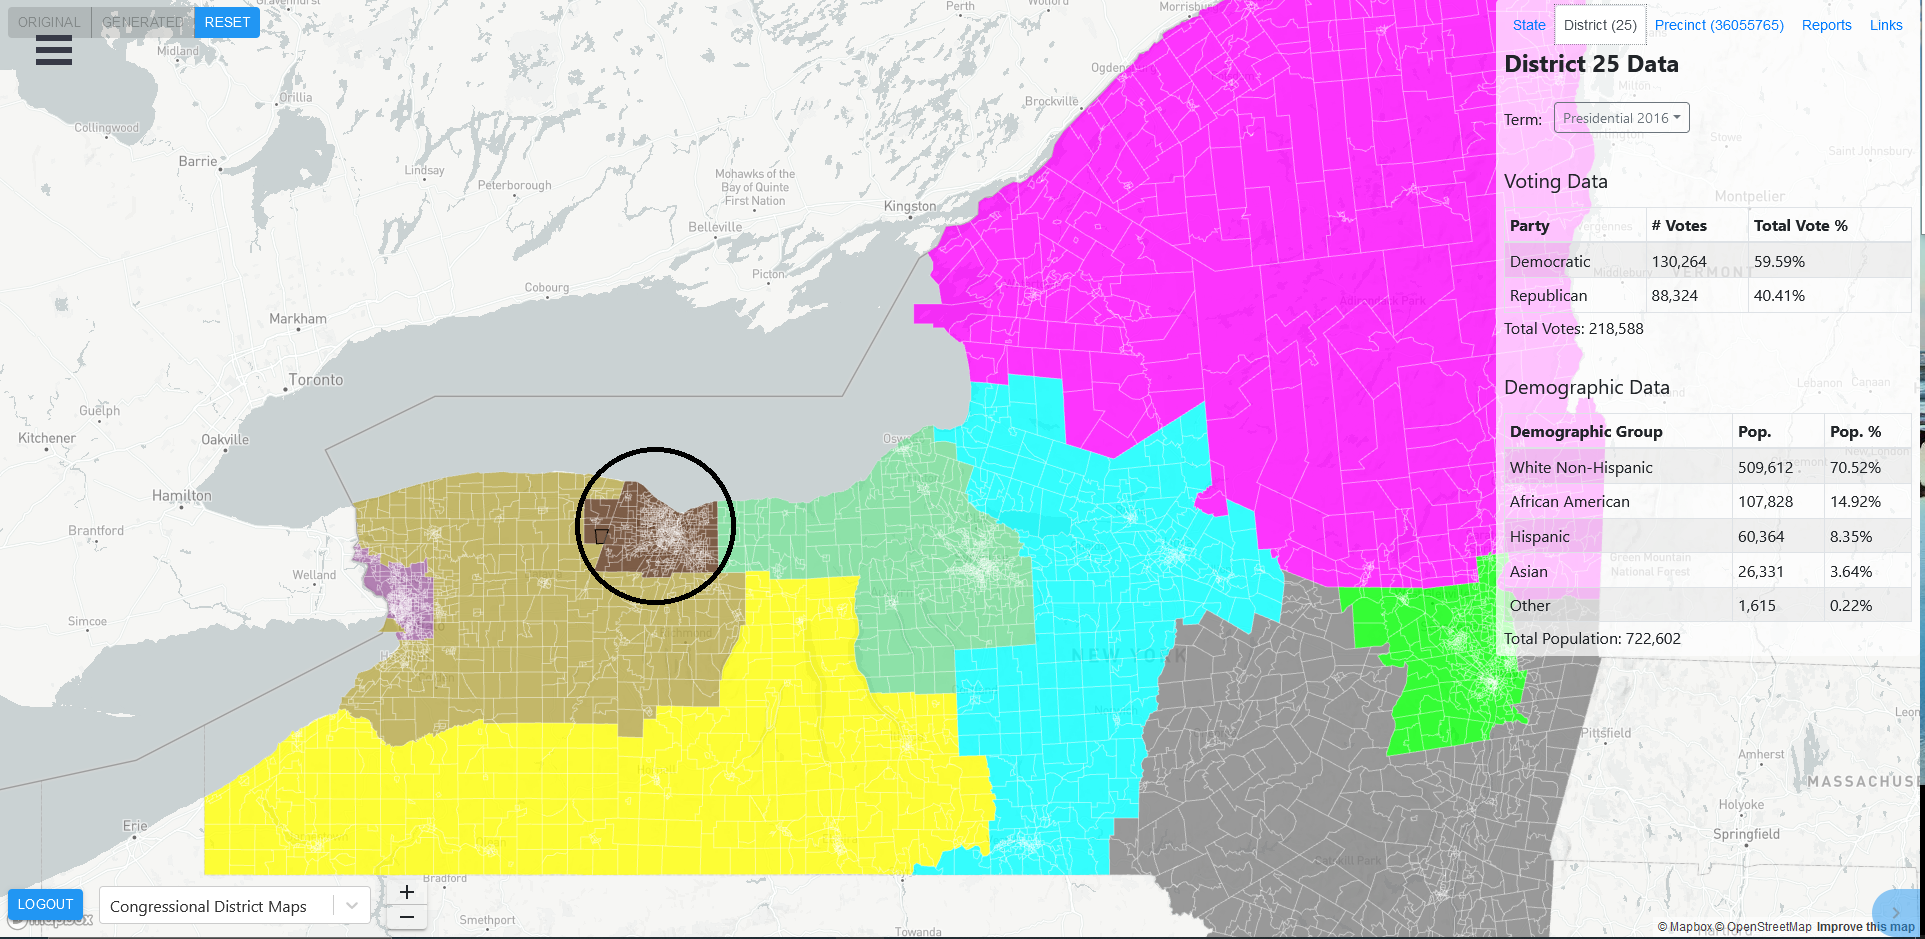
\includegraphics[width=\linewidth]{./figures/NY-25-BoundingCircle.png}
	\caption{NY-25 Bounding Circle}
	\label{fig:ny25boundingCircle}
\end{figure}

\begin{figure}[H]
	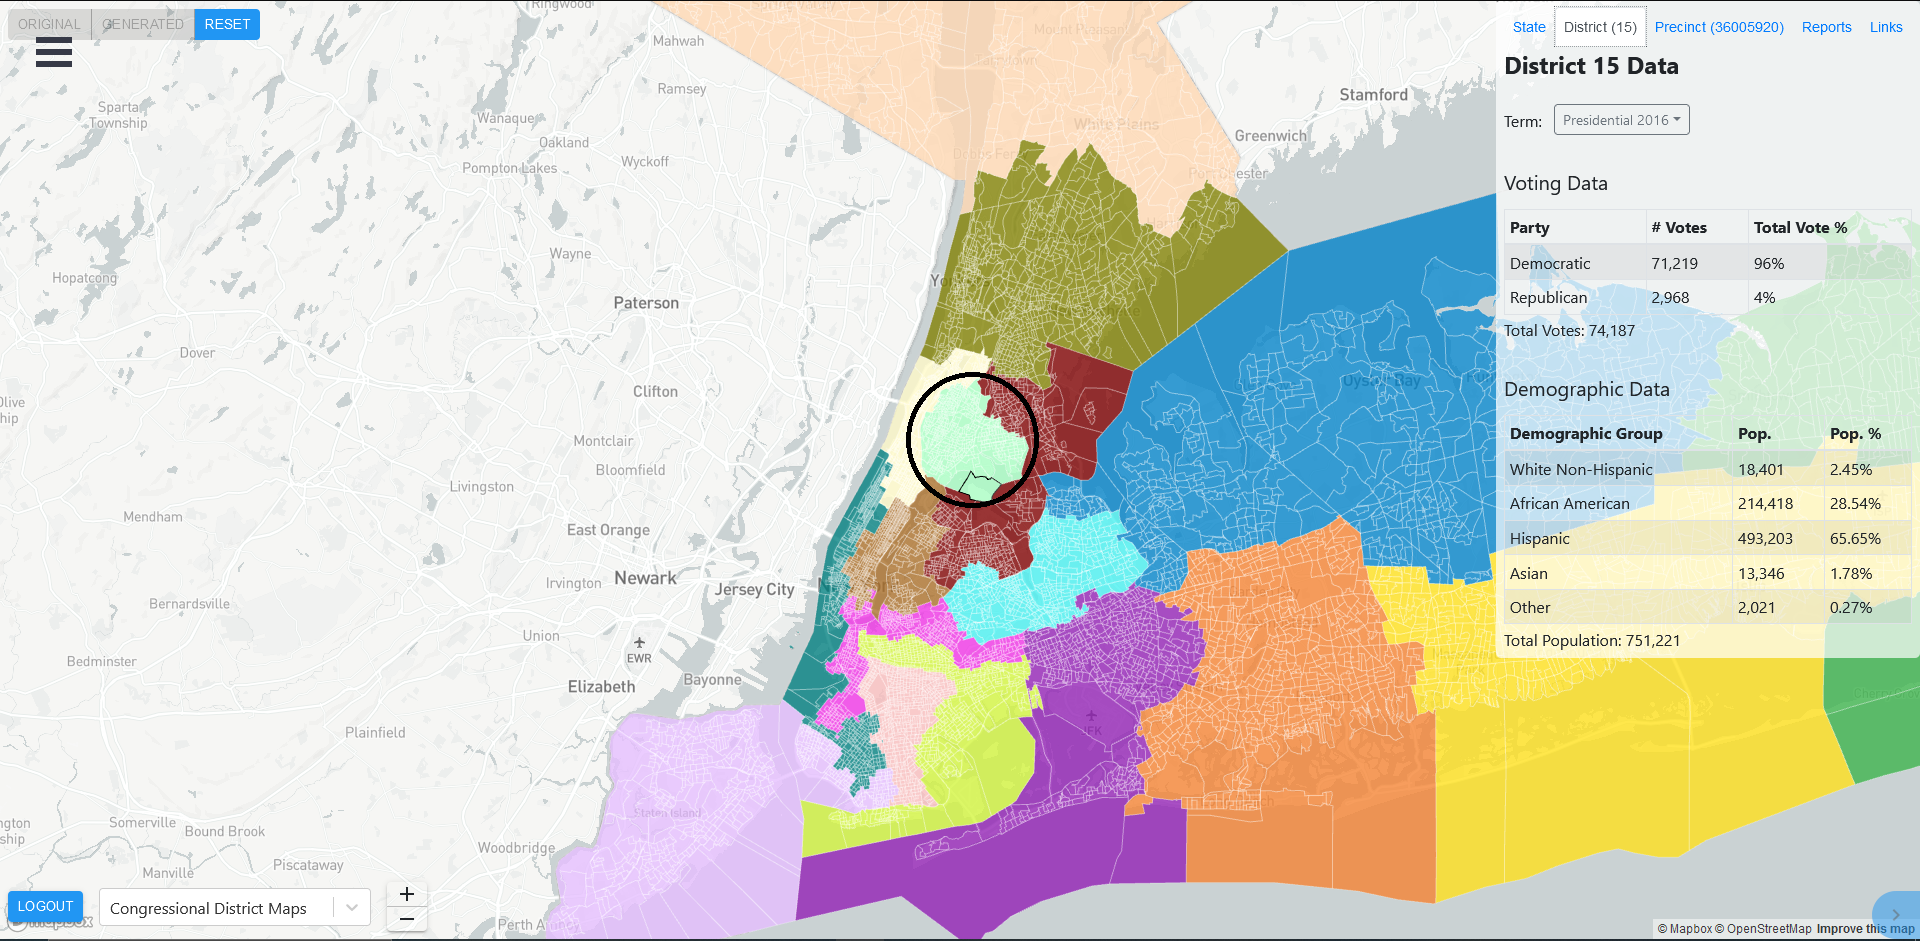
\includegraphics[width=\linewidth]{./figures/NY-15-BoundingCircle.png}
	\caption{NY-15 Bounding Circle}
	\label{fig:ny15boundingCircle}
\end{figure}

\begin{figure}[H]
	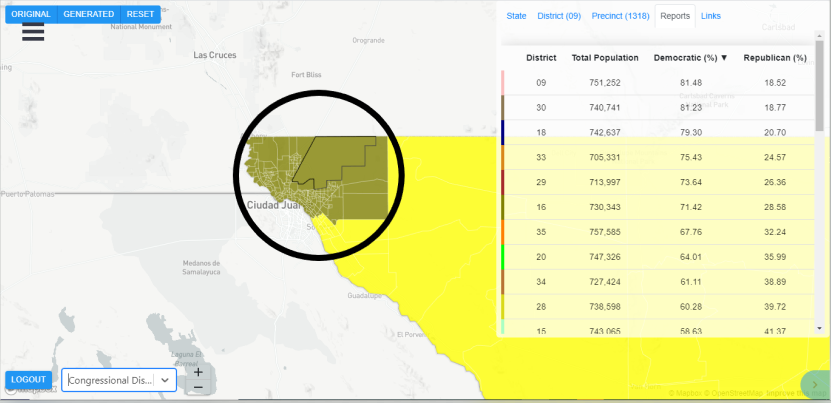
\includegraphics[width=\linewidth]{./figures/TX-16-BoundingCircle.png}
	\caption{TX-16 Bounding Circle}
	\label{fig:tx16boundingCircle}
\end{figure}

These districts are all centered around a major population hub. NY-25 is centered on Rochester, NY-15 is centered on the Bronx, and TX-16 is centered on El Paso. These districts geometrically all look compact and we believe that no one would considered them abnormal in any sense. This explains the high Polsby Popper score and also partially explains the high Fatness score. 

Specifically for the example of TX-16 which takes advantage of being small and densely populated with sparsely populated districts and state/country borders around, along with straight, perpendicular borders for most of its contour. It is a very Democratic area surrounded by moderately Republican areas, but it forms a coherent district encompassing one city and its direct surroundings, and contains all but the southernmost part of El Paso County, making it a very reasonable district. It is a similar story for the other districts.

\begin{figure}[H]
	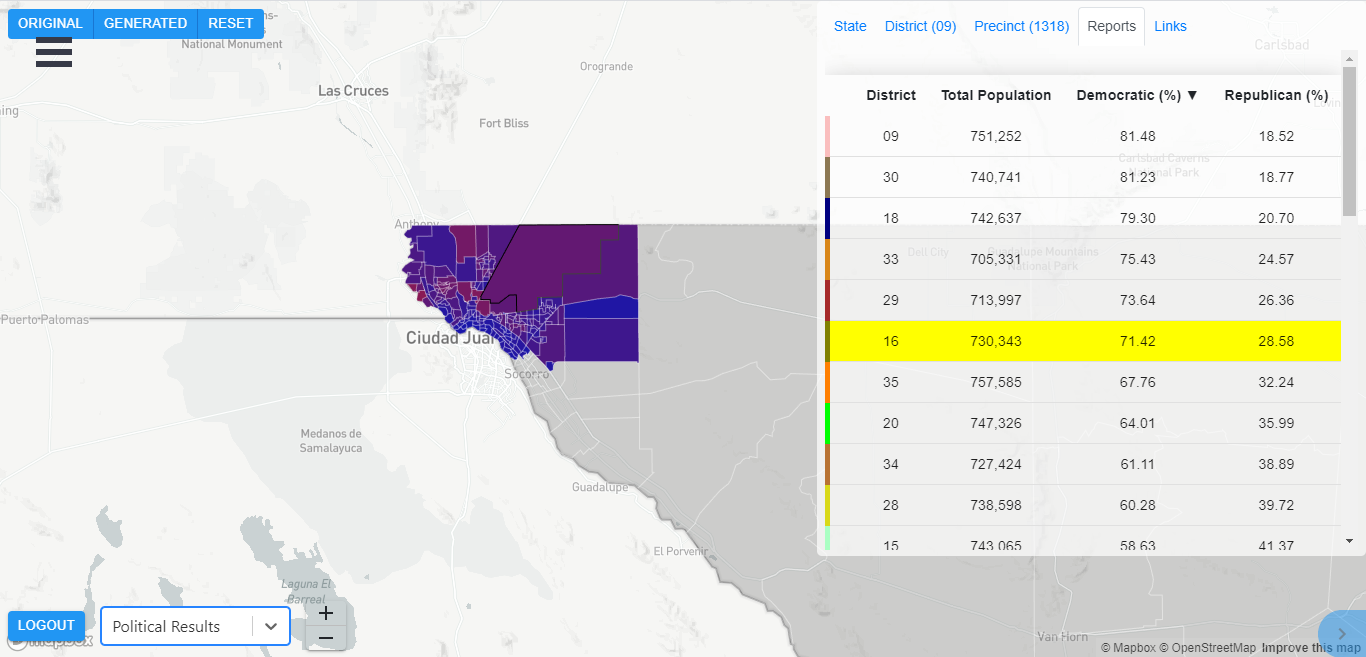
\includegraphics[width=\linewidth]{./figures/TX-16.png}
	\caption{TX-16}
	\label{fig:tx16border}
\end{figure}

\begin{figure}[H]
	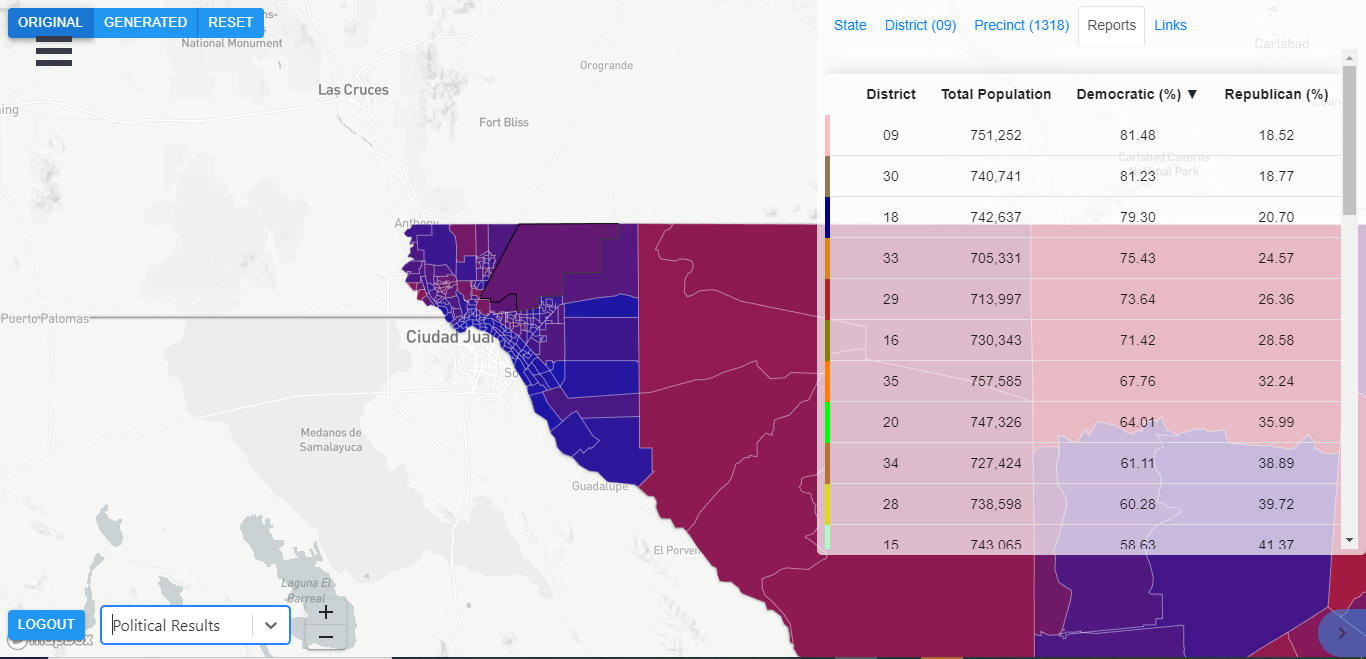
\includegraphics[width=\linewidth]{./figures/TX-16-SurroundingArea.png}
	\caption{TX-16 Political Results}
	\label{fig:tx16political}
\end{figure}

We now move onto the extremeties in the second quadrant. Specifically, many districts in Ohio form a cluster with low a Polsby Popper score and yet a relatively high Fatness score.

\begin{figure}[H]
	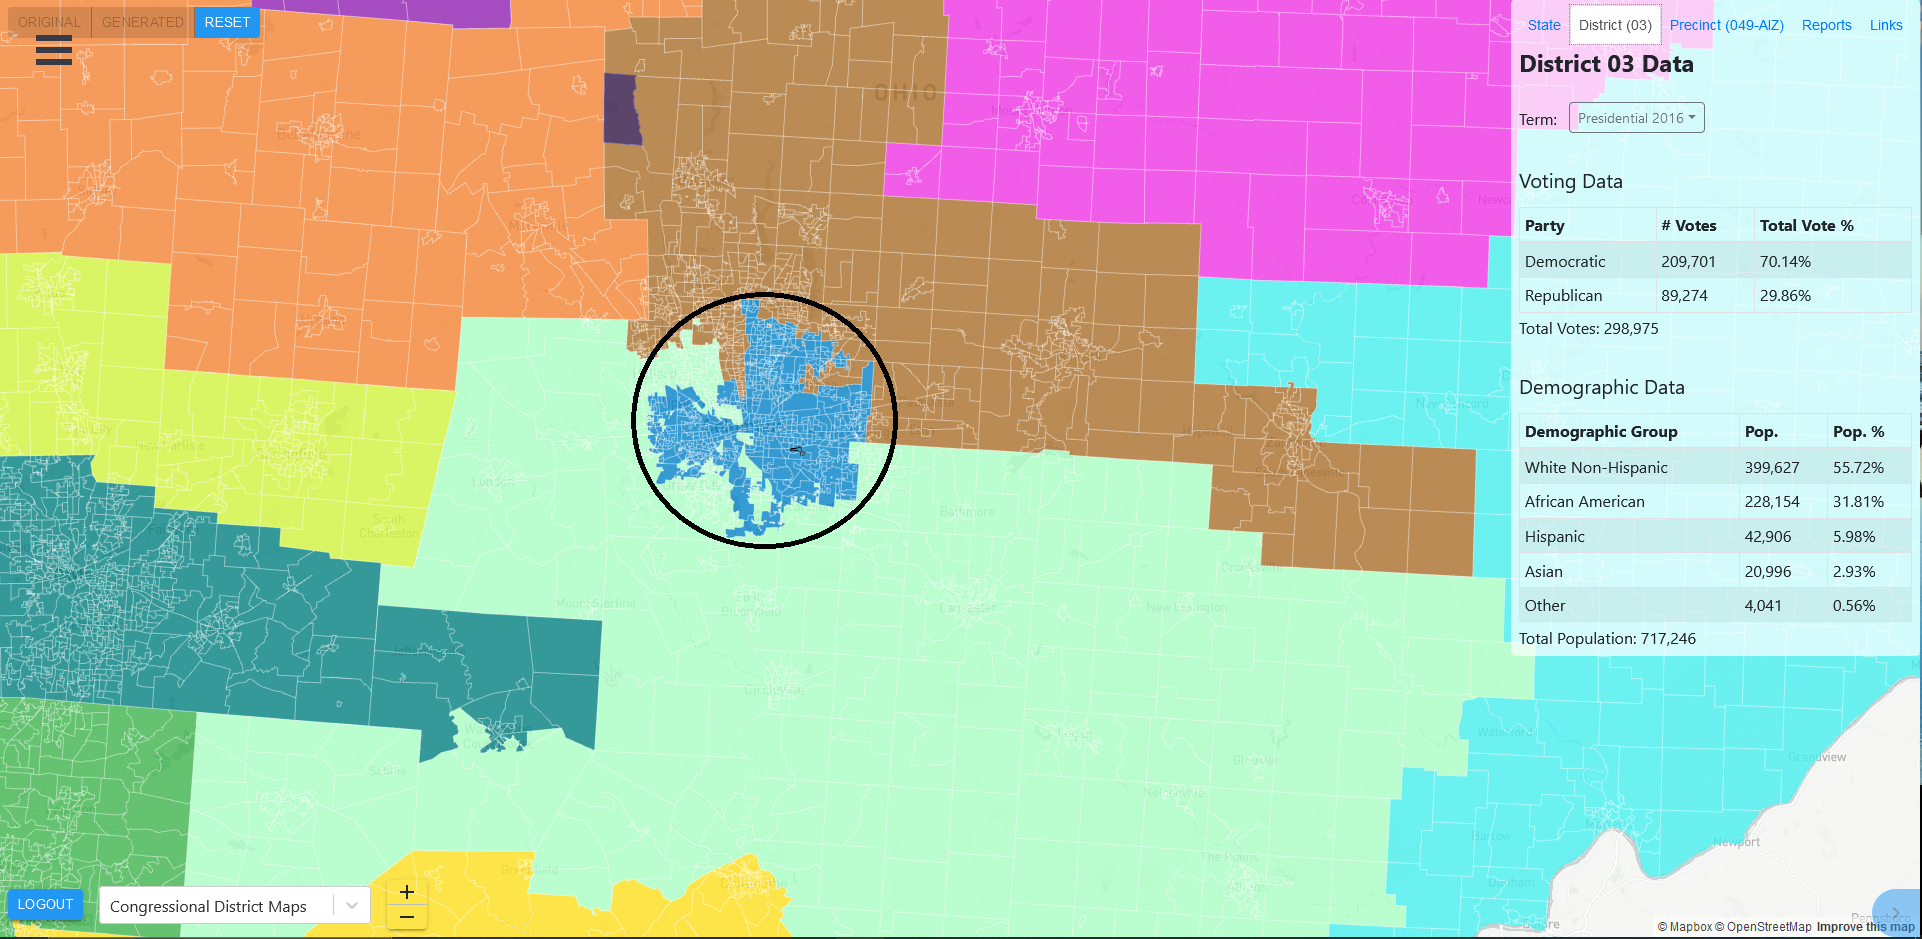
\includegraphics[width=\linewidth]{./figures/OH-03-BoundingCircle.png}
	\caption{OH-03 Bounding Circle}
	\label{fig:oh03boundingCircle}
\end{figure}

We will focus on Ohio's 3rd congressional district. It was named in a lawsuit specifically for gerrymandering. This is where our Fatness measure seems to fail as it gives a high score to the district while Polsby Popper gives it a low score. Polsby Popper's low score can be explained by the large perimeter that OH-03 has relative to its area. The fact of the matter is OH-03 is incredibly fractured on the city of Columbus. The fact that OH-03 is centered around the city of Columbus is also the reason why it scores highly in the Fatness measure.
%https://www.aclu.org/sites/default/files/field_document/complaint_timestamped.pdf

OH-11, the one with most of Cleveland, is heavily Democratic and connects two urban areas. The surrounding districts are barely Republican, and neighborhoods were carved carefully to ensure that this district would encompass as many Democrats as possible. Since Ohio’s map was drawn by a Republican state legislature, it is quite safe to assume that this is an attempt at gerrymandering. OH-03, in the heart of Columbus, suffers from the same issue: it is surrounded by two moderately Republican districts, OH-12 and OH-15, meaning that there is only one Democratic district in Columbus when there could be two with a different drawing.  While a potential excuse could be that this mostly follows the Columbus metropolitan area, it does not represent the will of the voters in the greater Columbus area quite fairly. 

\begin{figure}[H]
	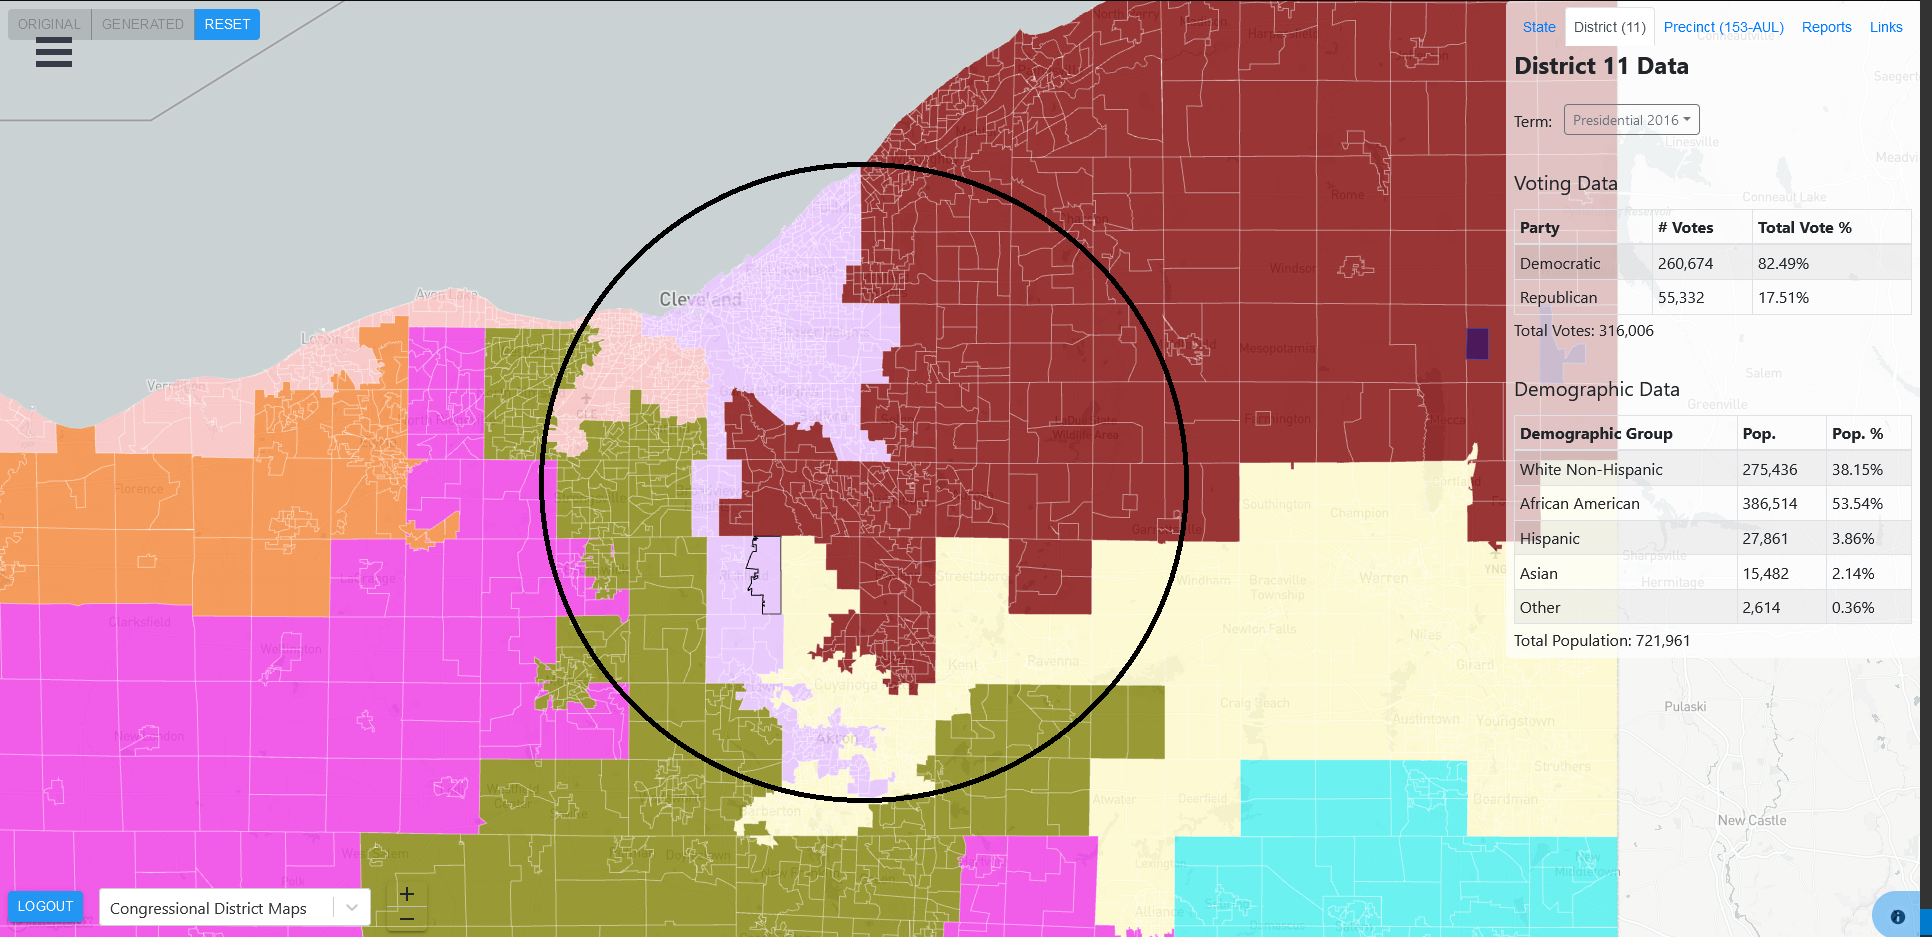
\includegraphics[width=\linewidth]{./figures/OH-11-BoundingCircle.png}
	\caption{OH-11 Bounding Circle}
	\label{fig:oh11boundingCircle}
\end{figure}


%Need to explain why Ohio 16 is average in the Fatness score

We can now skip ahead to the third quadrant. These are the districts often pointed out by opponents of gerrymandering as being “bad”, failing most standard measures for compactness.

\begin{figure}[H]
	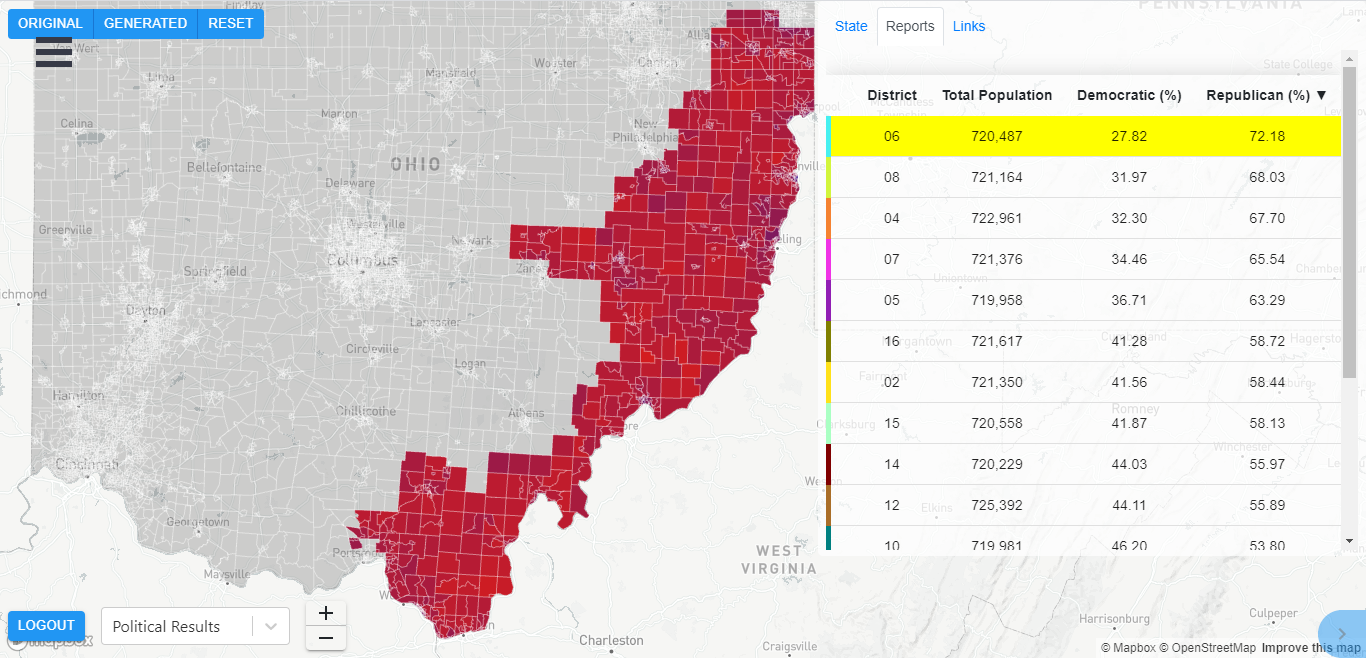
\includegraphics[width=\linewidth]{./figures/OH-06.png}
	\caption{Ohio District 06}
	\label{fig:oh06border}
\end{figure}

\begin{figure}[H]
	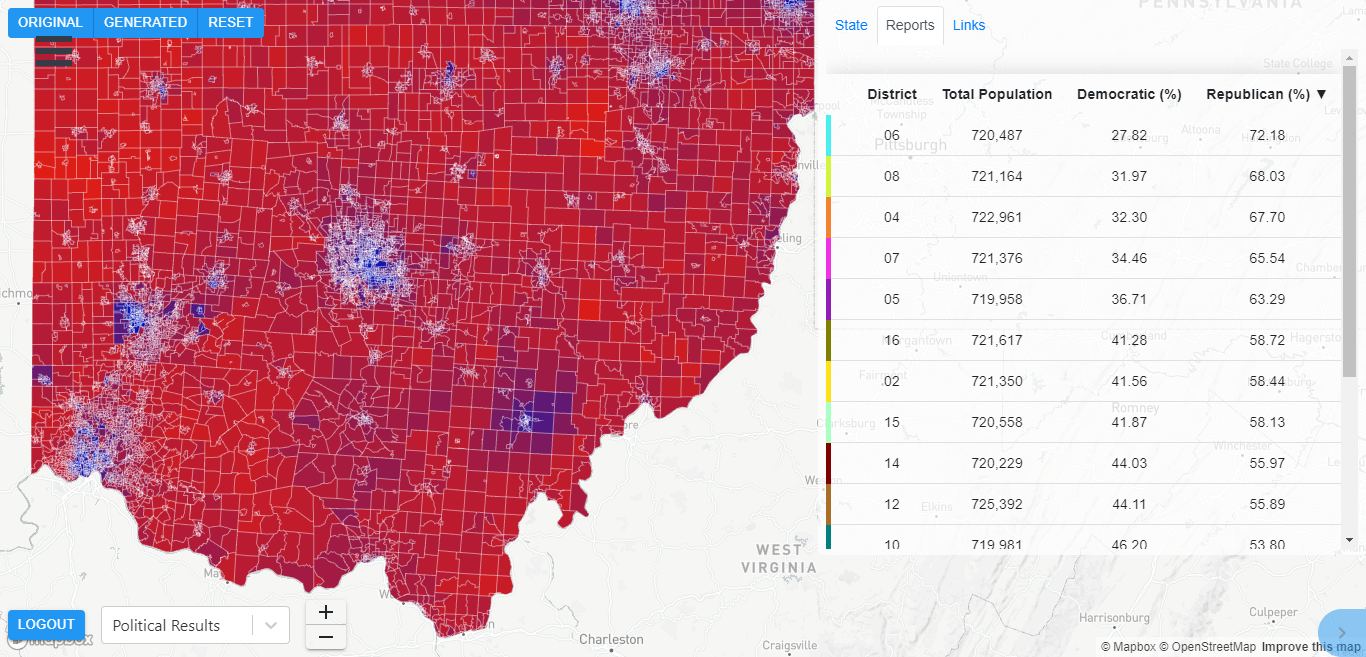
\includegraphics[width=\linewidth]{./figures/OH-06-SurroundingArea.png}
	\caption{OH-06 Political Results}
	\label{fig:oh06political}
\end{figure}

\begin{figure}[H]
	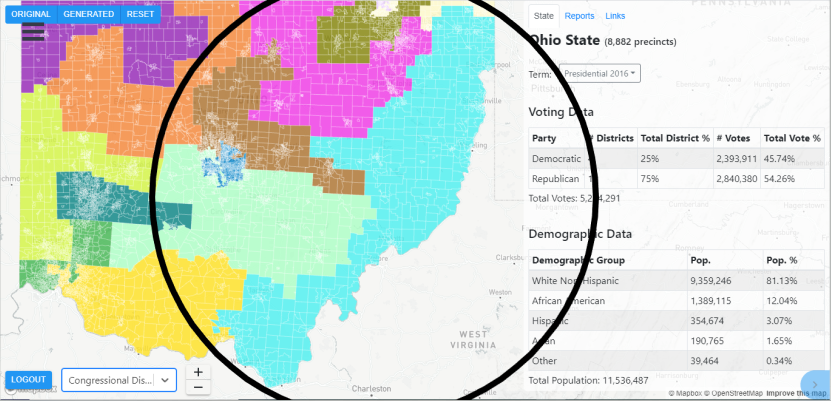
\includegraphics[width=\linewidth]{./figures/OH-06-BoundingCircle.png}
	\caption{OH-06 Bounding Circle}
	\label{fig:oh06boundingCircle}
\end{figure}

OH-06 is a good example of this: it covers all of Southeast Ohio, but is unnecessarily stretched out, with several indents both ways from neighboring districts. For example, Athens or Youngstown, places that lean Democratic, are barely out of the district. Once again in Ohio, OH-04 is also quite serpentine in shape and obviously avoids multiple areas, such as the indent made by OH-05, or the coast that is monopolized by OH-09 (it is worth mentioning that OH-09 is the only Democratic-leaning district of Northwest Ohio). As neighboring districts lean Republican like OH-04, we can see that small portions of urban areas such as Lorain or Strongsville were incorporated, but are not enough to switch the vote. What is currently Rep. Jim Jordan’s district clearly could instead have taken the large swaths of Republican land that create a hole in the middle of the district. It’s too bad this district is not in the other state that begins with an O, as this “duck” district would have been a good explanation for that state’s university’s mascot.

\begin{figure}[H]
	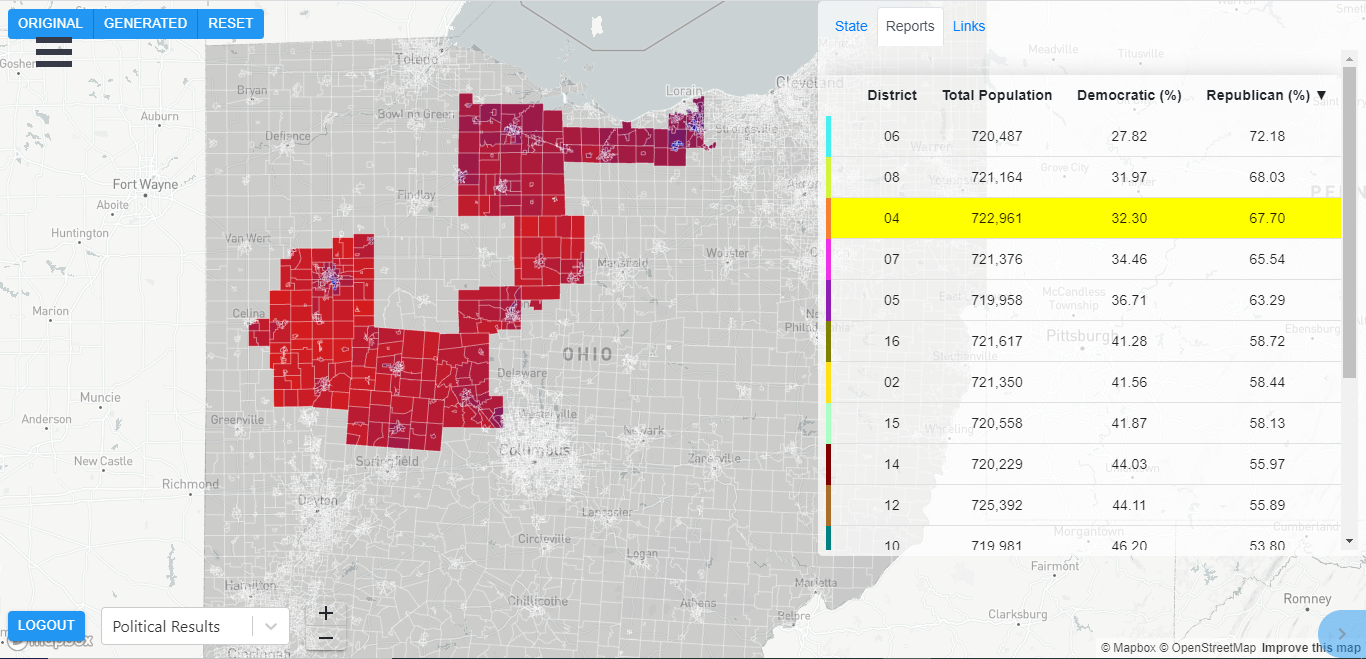
\includegraphics[width=\linewidth]{./figures/OH-04.png}
	\caption{Ohio District 04}
	\label{fig:oh04border}
\end{figure}

\begin{figure}[H]
	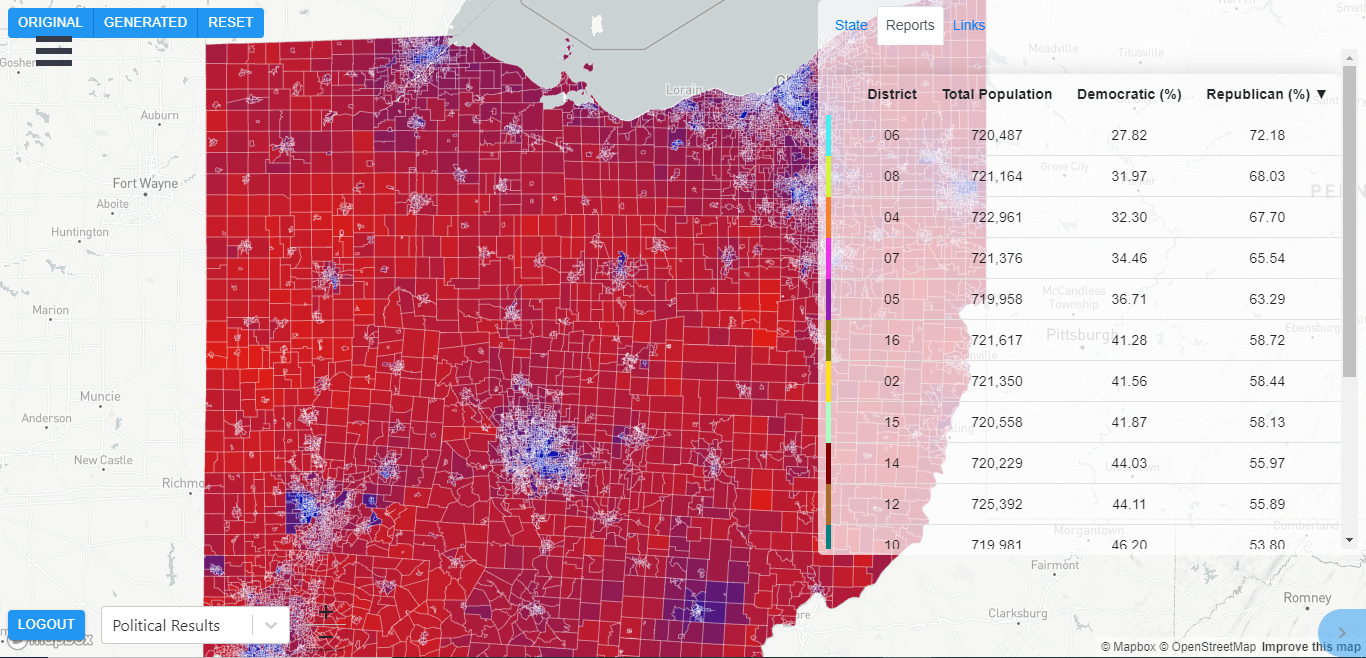
\includegraphics[width=\linewidth]{./figures/OH-04-SurroundingArea.png}
	\caption{OH-04 Political Results}
	\label{fig:oh04political}
\end{figure}

\begin{figure}[H]
	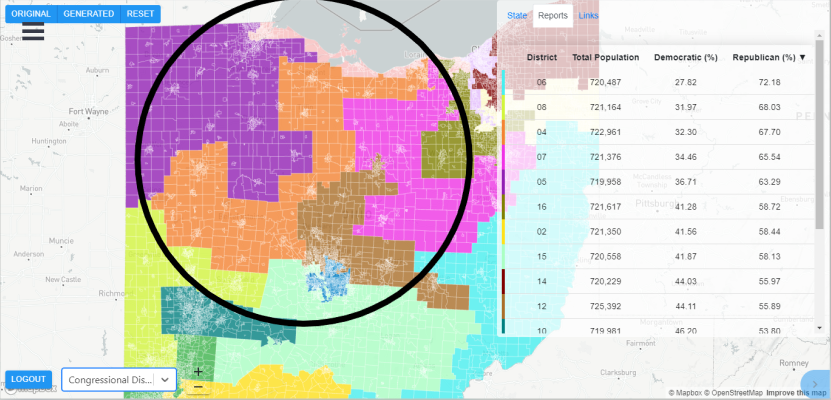
\includegraphics[width=\linewidth]{./figures/OH-04-BoundingCircle.png}
	\caption{OH-04 Bounding Circle}
	\label{fig:oh04boundingCircle}
\end{figure}

%Needs better explaination and better citation

As an aside: OH-04 has a very large prison and thousands of African American inmates that cannot vote. This also clearly does not respect county lines in the East (but look at OH-11, and Summit County, with four districts and no Congress representative…)
https://www.wksu.org/government-politics/2019-11-15/how-did-ohios-most-liberal-city-end-up-with-its-most-conservative-congressman

We will finally take a look at the fourth and last quadrant of the plot. It is sparcely populated and represents districts that score high in Polsby Popper but low in Fatness. We will look at NY-17, NY-18, NY-21, PA-08, and GA-09.

\begin{figure}[H]
	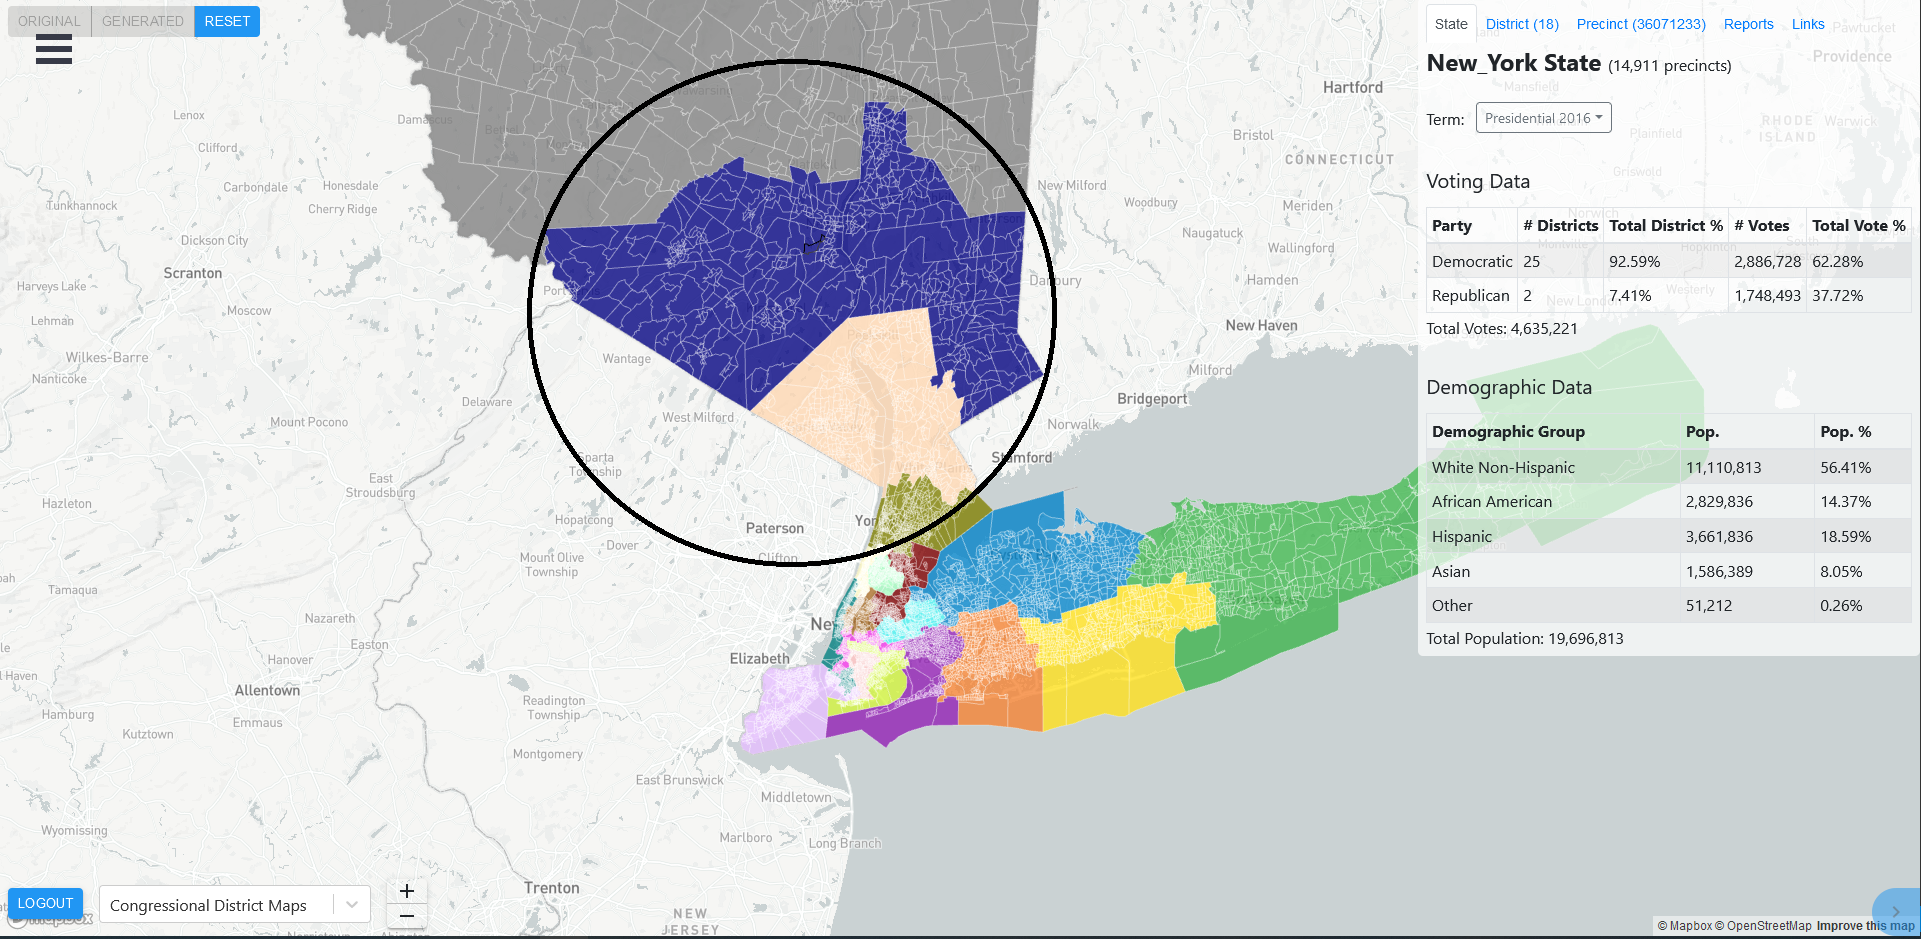
\includegraphics[width=\linewidth]{./figures/NY-18-BoundingCircle.png}
	\caption{NY-18 Bounding Circle}
	\label{fig:ny18boundingCircle}
\end{figure}

\begin{figure}[H]
	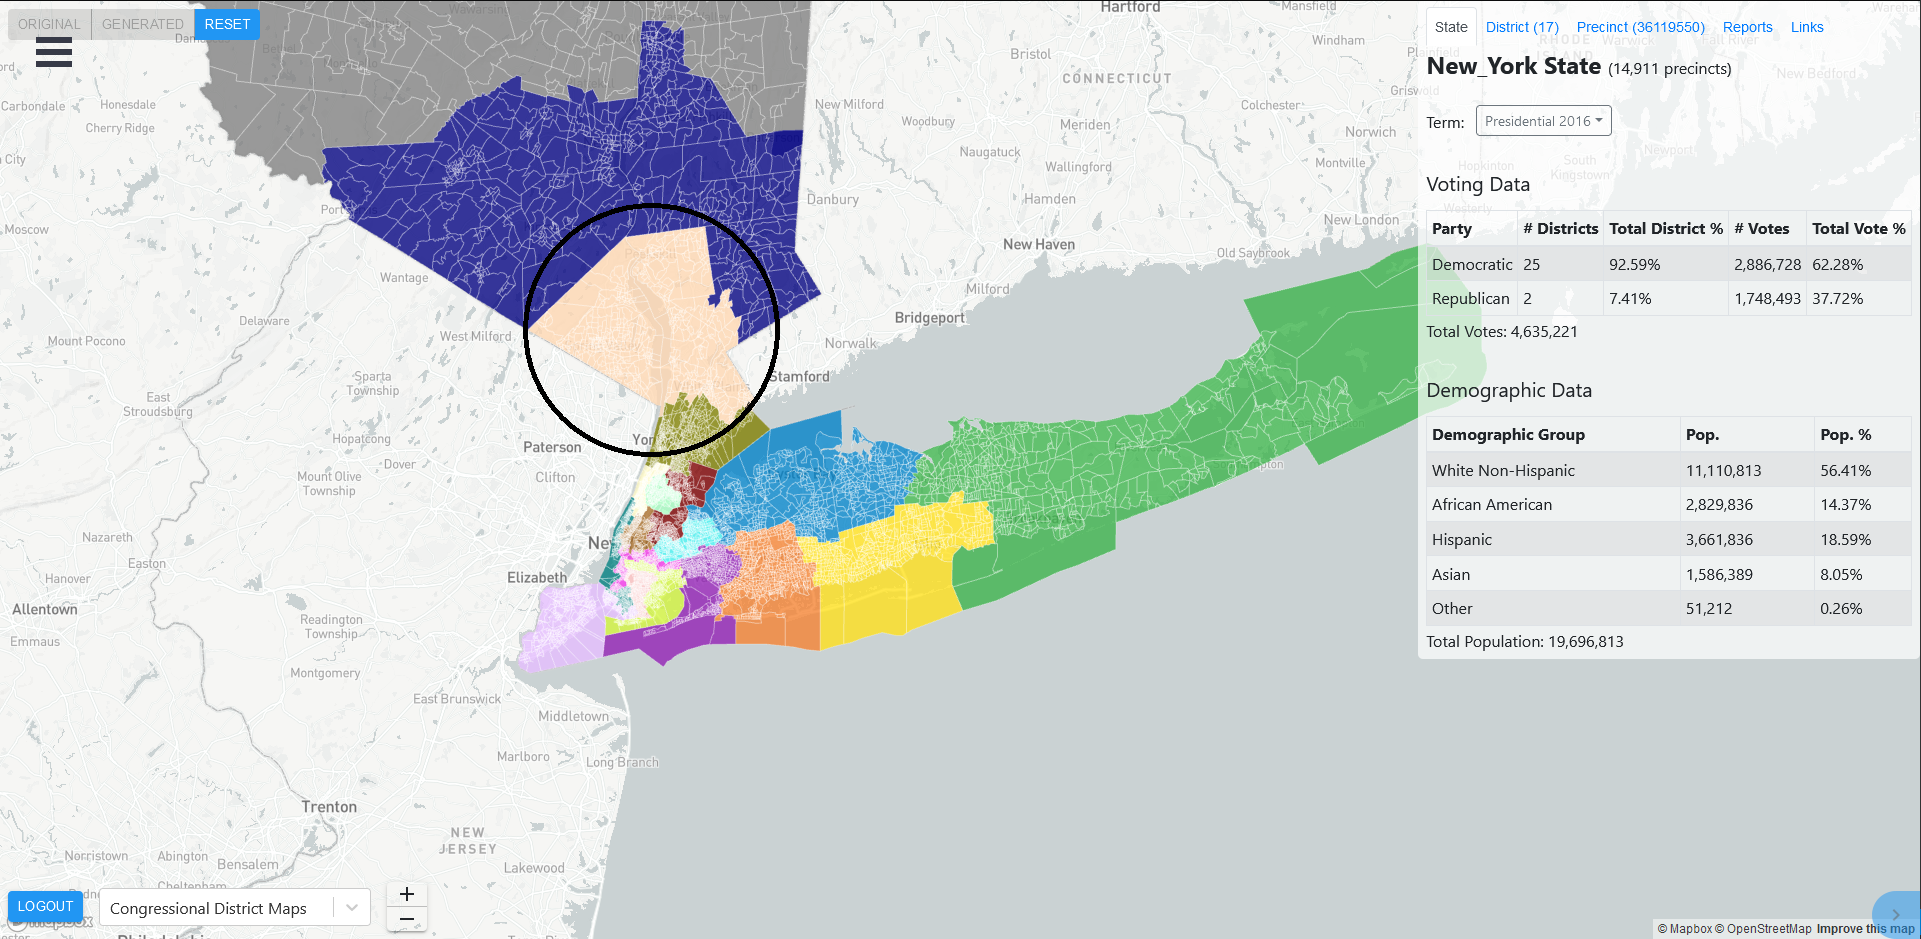
\includegraphics[width=\linewidth]{./figures/NY-17-BoundingCircle.png}
	\caption{NY-17 Bounding Circle}
	\label{fig:ny17boundingCircle}
\end{figure}

These two districts from New York have low fatness scores yet high Polsby Popper scores due to the unique shape of the state. These two districts are "funnel" shaped towards one of the most populous city in the entire country. Therefore, parts of the bounding circle enroach upon the city and its outer suburbs. This causes the fatness score to be low since it "misses" the more populous precincts of the state.

\begin{figure}[H]
	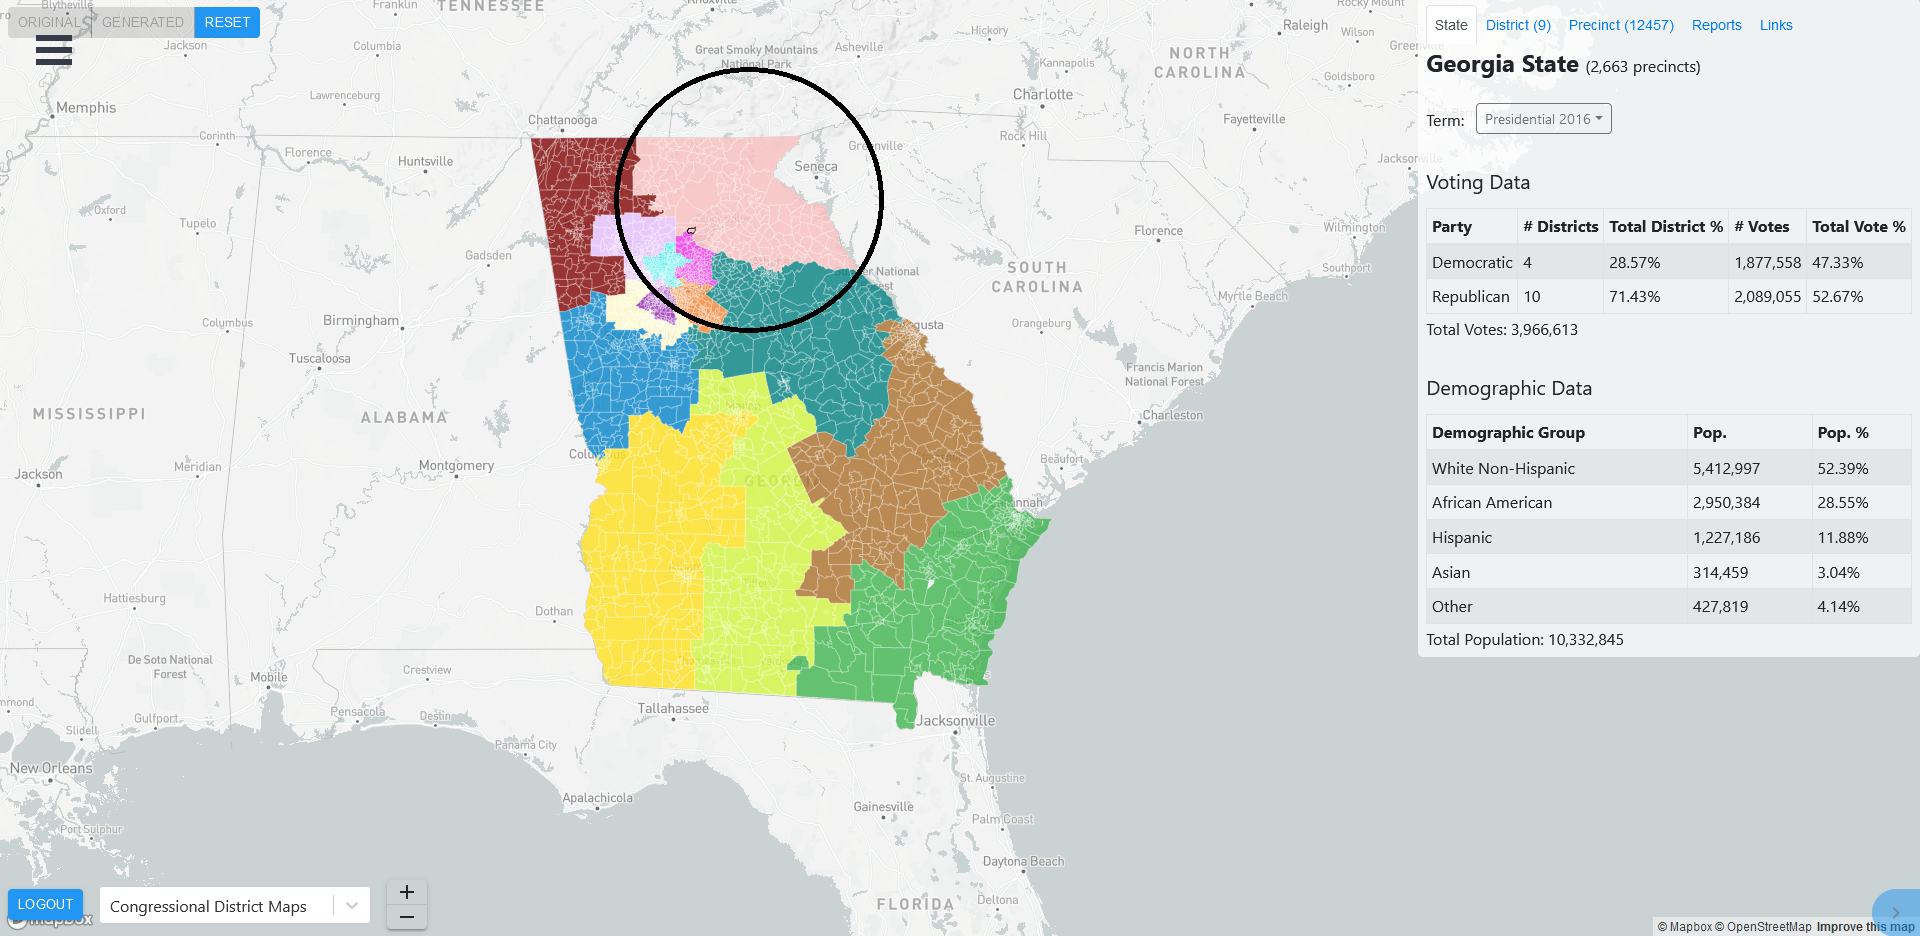
\includegraphics[width=\linewidth]{./figures/GA-09-BoundingCircle.png}
	\caption{GA-09 Bounding Circle}
	\label{fig:ga09boundingCircle}
\end{figure}

The same situation can be applied to Georgia's 9th congressional district. The "long" shape of GA-09 going from northwest to southeast causes its bounding circle to contain the city of Alanta. It is again a major population source. One thing to not is that although Alanta predominately leans towards the Democratic Party, GA-09 consistently leans Republican. It is one of the most pro-republican districts in the state of Georgia.

\begin{figure}[H]
	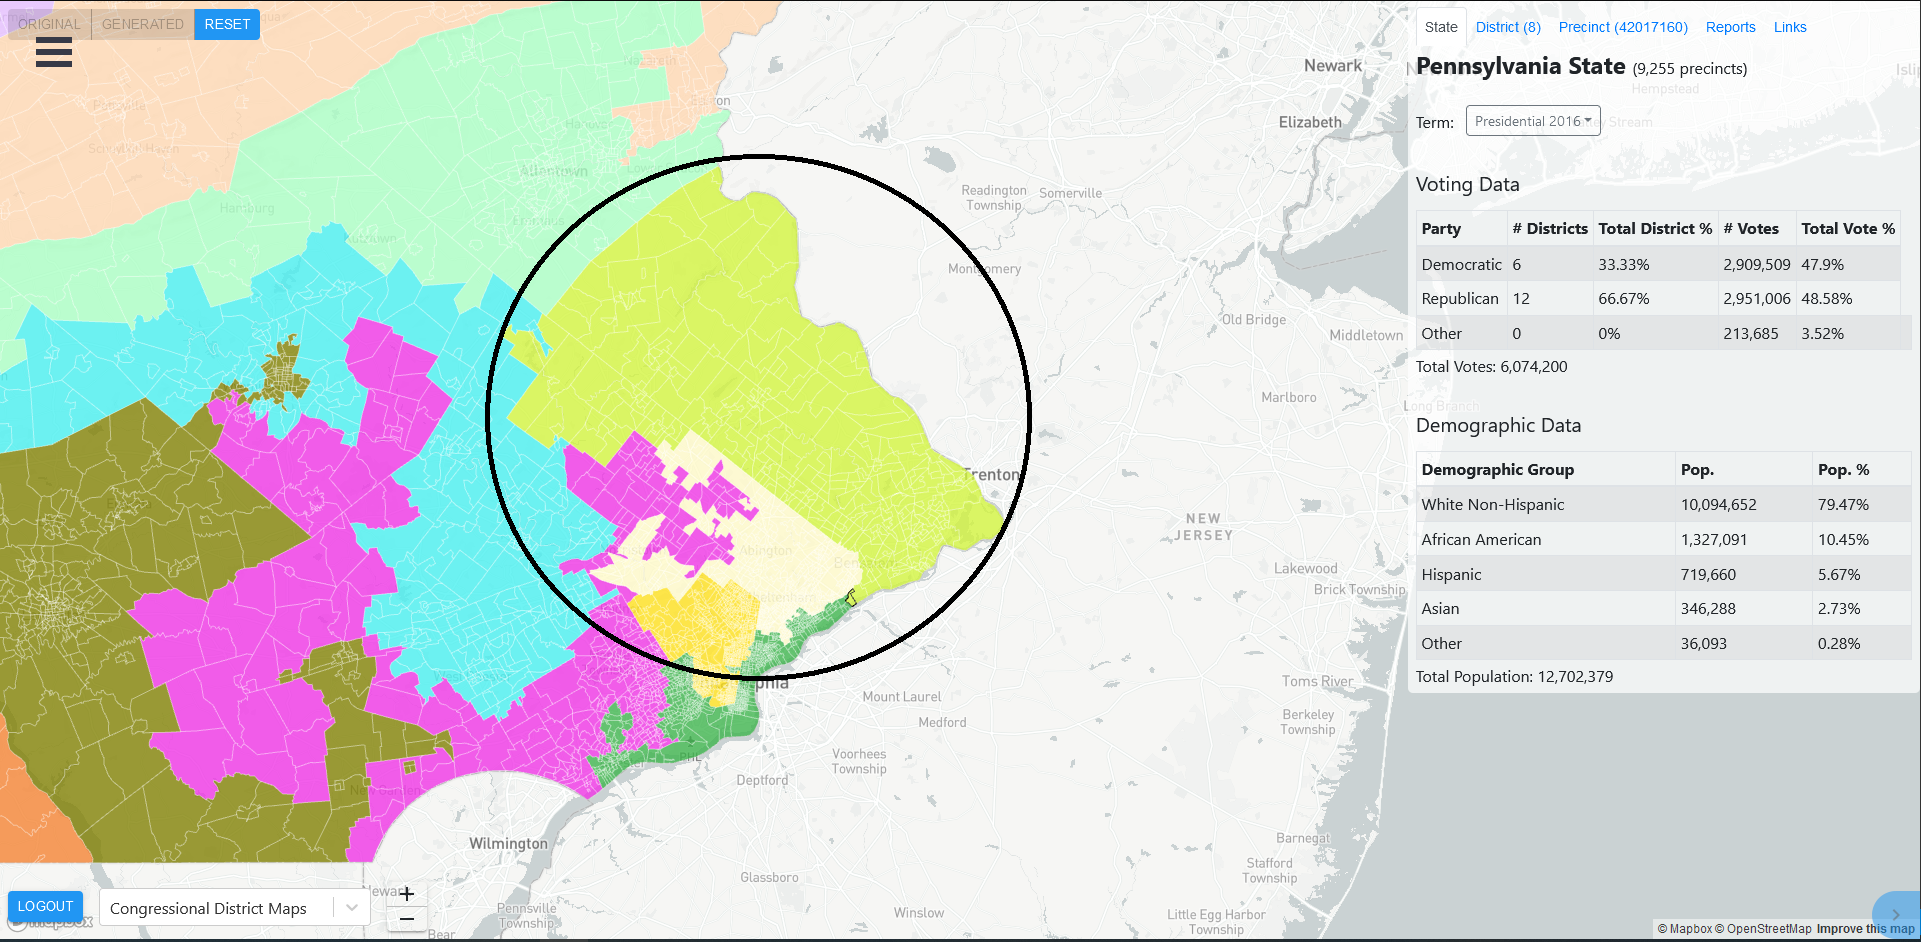
\includegraphics[width=\linewidth]{./figures/PA-08-BoundingCircle.png}
	\caption{PA-08 Bounding Circle}
	\label{fig:pa08boundingCircle}
\end{figure}

Finally, Pennsylvania's 8th congressional district tells us the same story as the past three districts. As one can see, PA-08 sits right outside of Philidelphia, but its bounding circle does not. This again causes the high population of Philidelphia to be just outside of the district's borders but within the bounding circle, thus causing the low fatness score. It is a recurring theme in this quadrant of the graph that these districts seem to be just outside of major population zones and is part of the state's borders.



Before concluding our work on the two measures, we will go to a somewhat miscellaneous example in California. CA-08 scores the worst fatness score across all ten states studied, and the Polsby-Popper score is mediocre as well. It is true that this is perhaps not the best district, however, its score is harmed by what is going on behind the district lines. While it does have a rather jagged western boundary and a rather long rectilinear shape, the fatness score is deserving of the deeper analysis. It is no coincidence that the worst fatness measure is in the most populous state, and specifically, one with both very densely and sparsely populated areas. The diameter of the bounding circle of this large district is almost the northeast border of the district - this means that besides northern California and the Bay Area, virtually all of California is within that bounding circle. The fatness score is close to 0.025, which would indicate that about a fortieth of the bounding circle population is within the district: this means there are about forty districts inside of this circle (note that since we do not consider populations outside of the state, this would be impossible in any other state)! 


\section{Future Considerations}
With all of these case studies, there are quite a few things we can say about these measures and their strengths and weaknesses compared to human perception - which is supposed to be the ultimate judge.

Polsby-Popper is good at catching districts that have unnecessarily long boundaries by penalizing them. As a result, districts with long straight lines tend to be favored. Something that is both positive and negative is that it does not depend on what is going on outside of the district, which means that we cannot see if population groups are avoided, but on the other hand, districts are not graded based on their size as a dilation of district by any strictly positive constant still yields the same score. However, sometimes, the border looks straight from a distance but is not on closer inspection: this can give unnecessarily low scores, unless the border is smoothened, a less straightforward and undebatable process than it may appear.

The population fatness measure devised, on the other hand, will “punish” long districts, and offers a solution to the issue of Polsby-Popper not taking into account what is happening right outside of the state. However, it has inherent downsides. For instance, as long as a bounding circle is small enough, the score will remain high: that is the case for OH-03 where several areas are removed from the bounding circle deeply down towards the middle, but this has a relatively limited effect on the fatness score. Additionally, this measure tends to favor districts on the edge of the state, since on at least one side, there is no population to consider. As a result, we suggest that there could instead be a computation of the arithmetic or geometric mean of the fatness scores, and that good plans should score above a certain threshold. The arithmetic mean (adding all scores) would favor good outliers in the state, and the geometric mean (multiplying all some) would strongly hinder bad outliers, so both systems have their (different) merits. More importantly, population fatness favors smaller districts, and those surrounding less populated areas. We saw this with examples such as TX-16 (El Paso is in the middle of the desert), OH-03 (with a good proportion of Columbus, with few of the suburbs concerned). However, larger districts tend to have more districts in their bounding circle, which automatically drop the population fatness score. In fact, this might create a political bias, since in general, Democratic congressional districts are more urban and smaller than their Republican counterparts. If we minimize the number of “nonfat” districts, we might crack Republican districts, but if we maximize the number of “fat” districts, we would pack Democrats. There are still many more questions to be answered, but as in other instances, they might show political bias. 


\bibliographystyle{unsrt}
\bibliography{citations}

\end{document}